% \documentclass[journal]{vgtc}                % final (journal style)
%\documentclass[review,journal]{vgtc}         % review (journal style)
%\documentclass[widereview]{vgtc}             % wide-spaced review
\documentclass[preprint,journal]{vgtc}       % preprint (journal style)

%% Uncomment one of the lines above depending on where your paper is
%% in the conference process. ``review'' and ``widereview'' are for review
%% submission, ``preprint'' is for pre-publication, and the final version
%% doesn't use a specific qualifier.

%% Please use one of the ``review'' options in combination with the
%% assigned online id (see below) ONLY if your paper uses a double blind
%% review process. Some conferences, like IEEE Vis and InfoVis, have NOT
%% in the past.

%% Please note that the use of figures other than the optional teaser is not permitted on the first page
%% of the journal version.  Figures should begin on the second page and be
%% in CMYK or Grey scale format, otherwise, colour shifting may occur
%% during the printing process.  Papers submitted with figures other than the optional teaser on the
%% first page will be refused. Also, the teaser figure should only have the
%% width of the abstract as the template enforces it.

%% These few lines make a distinction between latex and pdflatex calls and they
%% bring in essential packages for graphics and font handling.
%% Note that due to the \DeclareGraphicsExtensions{} call it is no longer necessary
%% to provide the the path and extension of a graphics file:
%% 
\includegraphics{diamondrule} is completely sufficient.
%%
\ifpdf%                                % if we use pdflatex
  \pdfoutput=1\relax                   % create PDFs from pdfLaTeX
  \pdfcompresslevel=9                  % PDF Compression
  \pdfoptionpdfminorversion=7          % create PDF 1.7
  \ExecuteOptions{pdftex}
  \usepackage{graphicx}                % allow us to embed graphics files
  \DeclareGraphicsExtensions{.pdf,.png,.jpg,.jpeg} % for pdflatex we expect .pdf, .png, or .jpg files
\else%                                 % else we use pure latex
  \ExecuteOptions{dvips}
  \usepackage{graphicx}                % allow us to embed graphics files
  \DeclareGraphicsExtensions{.eps}     % for pure latex we expect eps files
\fi%

%% it is recomended to use ``\autoref{sec:bla}'' instead of ``Fig.~\ref{sec:bla}''
\graphicspath{{figures/}{pictures/}{images/}{./}} % where to search for the images

\usepackage{microtype}                 % use micro-typography (slightly more compact, better to read)
\PassOptionsToPackage{warn}{textcomp}  % to address font issues with \textrightarrow
\usepackage{textcomp}                  % use better special symbols
\usepackage{mathptmx}                  % use matching math font
\usepackage{times}                     % we use Times as the main font
\renewcommand*\ttdefault{txtt}         % a nicer typewriter font
\usepackage{cite}                      % needed to automatically sort the references
\usepackage{tabu}                      % only used for the table example
\usepackage{booktabs}                  % only used for the table example
%% We encourage the use of mathptmx for consistent usage of times font
%% throughout the proceedings. However, if you encounter conflicts
%% with other math-related packages, you may want to disable it.

%% In preprint mode you may define your own headline.
%\preprinttext{To appear in IEEE Transactions on Visualization and Computer Graphics.}

%% If you are submitting a paper to a conference for review with a double
%% blind reviewing process, please replace the value ``0'' below with your
%% OnlineID. Otherwise, you may safely leave it at ``0''.

\onlineid{0}


%% declare the category of your paper, only shown in review mode
\vgtccategory{Research}
%% please declare the paper type of your paper to help reviewers, only shown in review mode
%% choices:
%% * algorithm/technique
%% * application/design study
%% * evaluation
%% * system
%% * theory/model
\vgtcpapertype{application}

\usepackage{dsfont}
\let\temp\rmdefault
\usepackage{mathpazo}
\let\rmdefault\temp

\usepackage{float}
\usepackage{subfigure}
\newcommand{\ds}{\displaystyle}
\newcommand{\nl}{\newline}
\newcommand{\eps}{\varepsilon}
\newcommand{\ssty}{\scriptstyle}
\newcommand{\bE}{\mathds{E}}
\newcommand{\cB}{\mathcal{B}}
\newcommand{\cF}{\mathcal{F}}
\newcommand{\cA}{\mathcal{A}}
\newcommand{\cM}{\mathcal{M}}
\newcommand{\cD}{\mathcal{D}}
\newcommand{\cP}{\mathcal{P}}
\newcommand{\cN}{\mathcal{N}}
\newcommand{\cL}{\mathcal{L}}
\newcommand{\cLN}{\mathcal{LN}}
\newcommand{\bP}{{\rm I\!P}}
\newcommand{\bQ}{\mathbb{Q}}
\newcommand{\bN}{{\rm I\!N}}
\newcommand{\bR}{\mathds{R}}
\newcommand{\bZ}{\mathbb{Z}}
\newcommand{\bC}{\mathbb{C}}
\newcommand{\ind}{\mathds{1}}
\newcommand{\data}{\mathcal{D}}
\newcommand{\bV}{\mathds{V}}

% \renewcommand{\boldsymbol}{\symbf}

\newcommand{\bfP}{\boldsymbol{P}}
\newcommand{\bfQ}{\boldsymbol{Q}}
\newcommand{\bfX}{\boldsymbol{X}}
\newcommand{\bfY}{\boldsymbol{Y}}
\newcommand{\bfZ}{\boldsymbol{Z}}
\newcommand{\bfM}{\boldsymbol{M}}
\newcommand{\bfU}{\boldsymbol{U}}

\newcommand{\bfz}{\boldsymbol{z}}
\newcommand{\bfm}{\boldsymbol{m}}
\newcommand{\bfw}{\boldsymbol{w}}
\newcommand{\bfv}{\boldsymbol{v}}
\newcommand{\bfu}{\boldsymbol{u}}
\newcommand{\bfx}{\boldsymbol{x}}
\newcommand{\bfy}{\boldsymbol{y}}
\newcommand{\bfb}{\boldsymbol{b}}
\newcommand{\bfa}{\boldsymbol{a}}
\newcommand{\bfp}{\boldsymbol{p}}
\newcommand{\bff}{\boldsymbol{f}}
\newcommand{\tbx}{\tilde{\bfx}}
\newcommand{\tby}{\tilde{\bfy}}
\newcommand{\tbf}{\tilde{\bff}}
\newcommand{\yst}{\boldsymbol{y_\star}}
\newcommand{\fst}{\boldsymbol{f_\star}}
\newcommand{\xst}{\boldsymbol{x_\star}}
\newcommand{\bfth}{\boldsymbol{\theta}}
\newcommand{\bfmu}{\boldsymbol{\mu}}
\newcommand{\bfxi}{\boldsymbol{\xi}}
\newcommand{\bfsg}{\boldsymbol{\sigma}}


\newcommand{\htheta}{\hat{\theta}}
\newcommand{\poi}{\text{Poisson}}
% \newcommand{\var}{\text{Var}}
\newcommand{\cov}{\text{Cov}}
\newcommand{\gama}{\text{Gama}}
\newcommand{\normal}{\text{Normal}}
\newcommand{\ig}{\text{Inverse-Gamma}}
\newcommand{\ber}{\text{Bernoulli}}
\newcommand{\jg}{\text{Jg}}
\newcommand{\st}{\text{ s.t. }}
\newcommand{\otw}{\text{ otherwise }}
\newcommand{\sge}{\sigma_e^2}
\newcommand{\sgt}{\sigma_\theta^2}
\newcommand{\byi}{\bar{y}_i}
\newcommand{\gp}{\mathcal{GP}}

\newcommand{\dU}{\mathcal{U}}

%% Paper title.
\title{Gaussian Processes Visual Tool}

%% This is how authors are specified in the journal style

%% indicate IEEE Member or Student Member in form indicated below
\author{Eduardo Adame Salles}
\authorfooter{
%% insert punctuation at end of each item
\item
 Eduardo Adame is with the School of Applied Mathematics at the Getulio Vargas Foundation. E-mail: eduardo.salles@fgv.br.
}

%other entries to be set up for journal
\shortauthortitle{Adame: Global Illumination for Fun and Profit}
%\shortauthortitle{Firstauthor \MakeLowercase{\textit{et al.}}: Paper Title}

%% Abstract section.
\abstract{
  This paper presents the Gaussian Processes Visual Tool, an interactive tool for visualizing Gaussian Processes (GPs). The tool combines the power of Svelte, D3.js, Flask, and GPyTorch to provide a flexible and user-friendly interface. With the Gaussian Processes Visual Tool, users can visualize and understand GPs, make observations, and explore various kernel functions. The tool offers simulation options, allowing users to set axis parameters, likelihood variance, and even upload custom datasets. It stands out for its aesthetic design, comprehensive functionalities, and the integration of multiple important technologies. The Gaussian Processes Visual Tool fills a gap by offering a beautiful and useful tool that combines all essential GP functions in one place. The tool is publicly available on GitHub, enabling researchers and practitioners to employ it for GP visualization, experimentation, and education.
} % end of abstract

%% Keywords that describe your work. Will show as 'Index Terms' in journal
%% please capitalize first letter and insert punctuation after last keyword
\keywords{ Gaussian Processes, visualization, interactive tool, Svelte, D3.js, Flask, GPyTorch, regression.}

%% ACM Computing Classification System (CCS). 
%% See <http://www.acm.org/class/1998/> for details.
%% The ``\CCScat'' command takes four arguments.

\CCScatlist{ % not used in journal version
 \CCScat{K.6.1}{Management of Computing and Information Systems}%
{Project and People Management}{Life Cycle};
 \CCScat{K.7.m}{The Computing Profession}{Miscellaneous}{Ethics}
}

%% Uncomment below to include a teaser figure.
\teaser{
  \centering
  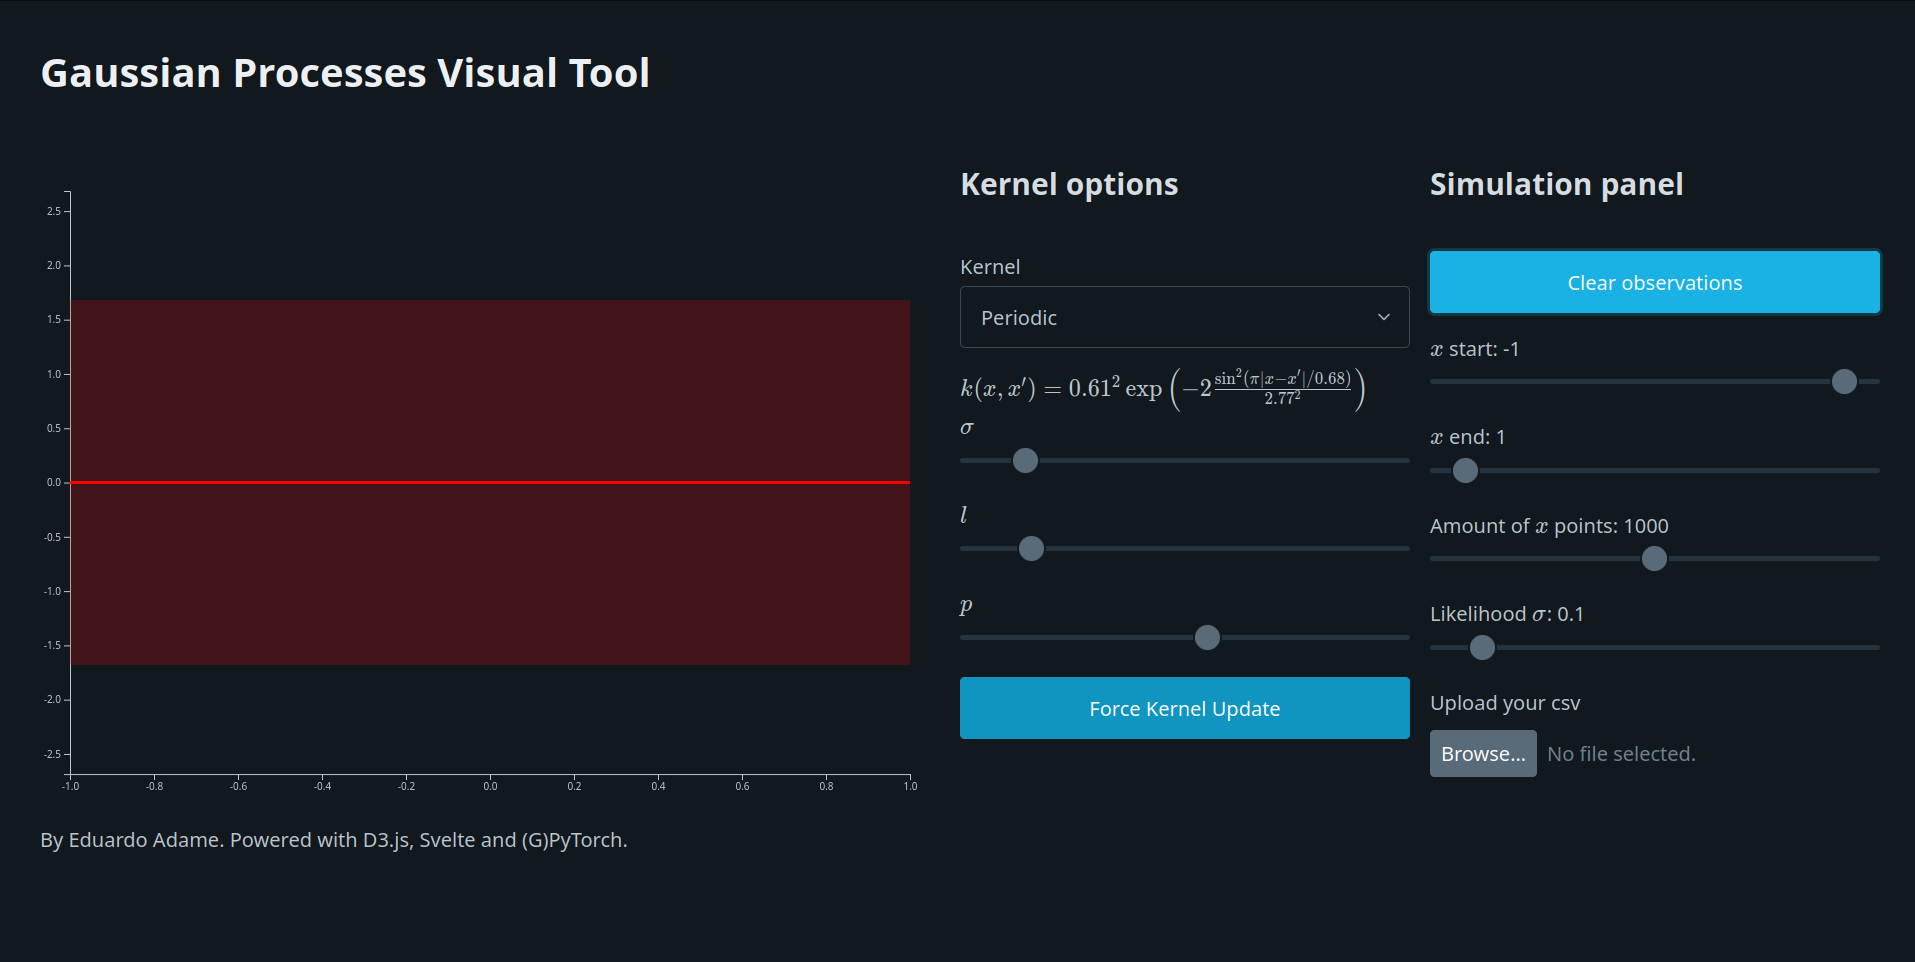
\includegraphics[width=\linewidth]{../imgs/overall.png}
  \caption{In the Clouds: Vancouver from Cypress Mountain. Note that the teaser may not be wider than the abstract block.}
	\label{fig:teaser}
}

%% Uncomment below to disable the manuscript note
%\renewcommand{\manuscriptnotetxt}{}

%% Copyright space is enabled by default as required by guidelines.
%% It is disabled by the 'review' option or via the following command:
% \nocopyrightspace

\vgtcinsertpkg

%%%%%%%%%%%%%%%%%%%%%%%%%%%%%%%%%%%%%%%%%%%%%%%%%%%%%%%%%%%%%%%%
%%%%%%%%%%%%%%%%%%%%%% START OF THE PAPER %%%%%%%%%%%%%%%%%%%%%%
%%%%%%%%%%%%%%%%%%%%%%%%%%%%%%%%%%%%%%%%%%%%%%%%%%%%%%%%%%%%%%%%%

\usepackage{multicol}

\begin{document}

%% The ``\maketitle'' command must be the first command after the
%% ``\begin{document}'' command. It prepares and prints the title block.

%% the only exception to this rule is the \firstsection command
\firstsection{Introduction}

\maketitle

%% \section{Introduction} %for journal use above \firstsection{..} instead

Gaussian Processes (GPs)~\cite{rasmussen2006gaussian} have gained significant attention in the field of machine learning and data analysis due to their ability to model complex and non-linear relationships while providing probabilistic predictions. GPs have found applications in various domains, including regression, classification, time series analysis, and Bayesian optimization. However, understanding and interpreting GP models can be challenging, requiring effective visualization techniques and interactive tools.

The motivation behind developing the Gaussian Processes Visual Tool stems from the need for a user-friendly and intuitive tool that enables users to visualize and explore GP models efficiently. Traditional methods often fall short in providing a comprehensive understanding of GP models, hindering their widespread adoption. By addressing these challenges, the tool aims to democratize the usage of GPs and empower practitioners in leveraging their potential.

\subsection{Objectives and Scope of the Tool}

The main objective of the Gaussian Processes Visual Tool is to provide an interactive and user-friendly interface for visualizing and analyzing Gaussian Process models. The tool aims to facilitate the exploration and understanding of GP models by enabling users to interact with the data, visualize model predictions, and gain insights into the underlying patterns and uncertainties.

The tool's scope encompasses several key features and functionalities. Users can visualize the posterior distribution of the latent function $f$ in real-time. By clicking anywhere on the visualization, users can make observations and update the posterior distribution accordingly. This dynamic interaction allows users to explore the effects of observations on the model predictions and uncertainties.

The tool offers a list of different kernel functions to choose from, and users can set hyperparameters for each kernel. This flexibility enables users to customize the model's behavior and capture various types of patterns and relationships in the data.

In addition, the tool provides simulation options, allowing users to set the axis parameters, variance of the likelihood, and even upload their own datasets. This versatility empowers users to explore different scenarios and analyze their own data within the tool.

\subsection{Overview of the Technologies Used}

The development of the Gaussian Processes Visual Tool leverages several cutting-edge technologies to provide a powerful and intuitive user experience.

D3.js~\cite{d3js}, a popular JavaScript library for data visualization, is utilized to create dynamic and interactive visualizations that facilitate the exploration of GP models. Its rich set of tools and components enables the representation of complex data relationships in an intuitive and visually appealing manner.

Svelte~\cite{svelte}, a reactive web framework, is employed to build the frontend of the tool. With its reactive behavior and efficient update mechanisms, Svelte ensures smooth and responsive interactions, enhancing the user experience. It simplifies the development process by providing a component-based architecture and optimizing the rendering performance.

Flask~\cite{flask}, a lightweight web framework for Python, serves as the backend of the tool. It provides the necessary infrastructure for handling data uploads, preprocessing, and model training. Flask's simplicity and extensibility make it an ideal choice for developing web applications with Python.

PyTorch~\cite{paszke2019pytorch}, a powerful deep learning library, is integrated into the tool to enhance its modeling capabilities. By leveraging PyTorch, users can train and evaluate GP models with advanced techniques, such as deep Gaussian Processes or neural network embeddings, expanding the tool's potential applications.

GPyTorch~\cite{gardner2018gpytorch}, a Gaussian process library for deep learning, is integrated into the tool to enhance its modeling capabilities. GPyTorch leverages PyTorch's tensor computations and automatic differentiation to provide scalable and efficient GP inference. It enables flexible modeling choices and supports various advanced GP techniques, such as deep Gaussian Processes or neural network embeddings.

The Gaussian Processes Visual Tool stands out for its beautiful and user-friendly design, combining all essential functions in one place. It offers a seamless user experience, encompassing visualization of the posterior distribution, hyperparameter customization, simulation options, and dataset upload. The tool's comprehensive approach distinguishes it from existing projects that often focus on specific aspects of GP modeling.

\section{Background}

\subsection{Gaussian Processes}

Gaussian Processes (GPs) are powerful probabilistic models that have gained significant attention in the field of machine learning and data analysis. GPs provide a flexible framework for modeling complex relationships in data, making them well-suited for tasks such as regression, classification, time series analysis, and Bayesian optimization.

At its core, a Gaussian Process is defined as a collection of random variables, any finite number of which follow a joint Gaussian distribution. In simpler terms, a GP defines a distribution over functions rather than specific function values. Each point in the input space is associated with a random variable, and the covariance between these variables encodes the similarity between inputs.

GPs offer several advantages over traditional regression or classification models. First, GPs provide a non-parametric approach, meaning they do not assume a specific functional form for the underlying relationship. This flexibility allows GPs to capture complex and non-linear patterns in the data without being constrained by predefined assumptions.

Second, GPs provide probabilistic predictions, offering a measure of uncertainty for each prediction. This uncertainty estimation is particularly valuable in scenarios where decision-making relies on reliable confidence bounds or when the data is limited or noisy. The probabilistic nature of GPs also enables Bayesian inference, where prior knowledge and observed data can be combined to update beliefs about the underlying function.

Third, GPs can handle different types of inputs, including scalar values, vectors, or even structured data. This versatility makes GPs applicable to a wide range of domains and problem types.

To use GPs for regression or classification, a key step involves specifying a covariance function, often referred to as a kernel function. The choice of kernel function determines the assumed characteristics of the underlying function, such as smoothness, periodicity, or linearity. Popular kernel functions include the squared exponential, Matérn, and linear kernels.

In practice, Gaussian Processes can be trained using various inference methods, such as maximum likelihood estimation, Markov chain Monte Carlo (MCMC), or variational inference. The trained GP model can then be used for making predictions on new, unseen data points by leveraging the learned distribution over functions.

Overall, Gaussian Processes provide a flexible and probabilistic framework for modeling complex relationships in data. By capturing uncertainties and offering non-parametric modeling capabilities, GPs have found wide applications in machine learning, statistics, and various scientific domains.

\subsection{Gaussian Processes for Regression}

For our purposes, we focus on Gaussian Processes for regression tasks. In this setting, we assume that the observed data points are generated by a latent function $f$ with Gaussian noise $\epsilon$:

\begin{equation}
    y = f(x) + \epsilon
\end{equation}

where $x$ is the input and $y$ is the output. The goal of regression is to learn the underlying function $f$ from the observed data points and make predictions on new, unseen data points.

In the context of GPs, the latent function $f$ is assumed to follow a Gaussian Process:

\begin{equation}
    f \sim \mathcal{GP}(m(\cdot), k(\cdot, \cdot))
\end{equation}

where $m(\cdot)$ is the mean function and $k(\cdot, \cdot)$ is the covariance function, also known as the kernel function. The mean function $m(\cdot)$ is often assumed to be zero, and the kernel function $k(\cdot, \cdot)$ is used to encode the assumed characteristics of the underlying function, such as smoothness, periodicity, or linearity.

Given a set of observed data points $\mathcal{D} = \{(x_i, y_i)\}_{i=1}^N$, the goal is to learn the posterior distribution over functions $p(f|\mathcal{D})$. This posterior distribution can be used to make predictions on new, unseen data points $x^*$:

\begin{equation}
    p(y^*|x^*, \mathcal{D}) = \int p(y^*|x^*, f) p(f|\mathcal{D})\ df
\end{equation}

where $p(y^*|x^*, f)$ is the likelihood function, and $p(f|\mathcal{D})$ is the posterior distribution over functions. The posterior distribution $p(f|\mathcal{D})$ is a Gaussian distribution with mean $\mu$ and covariance $\Sigma$:

\begin{equation}
    p(f|\mathcal{D}) = \mathcal{N}(\mu, \Sigma)
\end{equation}
  
  where $\mu = K(X, X)K(X, X)^{-1}y$ and $\Sigma = K(X, X) - K(X, X)K(X, X)^{-1}K(X, X)$.

\subsection{Kernels for Gaussian Processes}

The choice of kernel function determines the assumed characteristics of the underlying function. For example, the squared exponential kernel encodes the assumption that the underlying function is smooth, while the Matérn kernel encodes the assumption that the underlying function is not smooth.

They must follow some properties to be valid kernels. For example, a valid kernel must be symmetric, positive semi-definite, and must satisfy the Mercer's condition. A kernel $k(\cdot, \cdot)$ is symmetric if $k(x, y) = k(y, x)$ for all $x, y \in \mathcal{X}$. A kernel $k(\cdot, \cdot)$ is positive semi-definite if for any finite set of points $x_1, \dots, x_n \in \mathcal{X}$, the corresponding kernel matrix $K$ is positive semi-definite. A kernel $k(\cdot, \cdot)$ satisfies the Mercer's condition if for any finite set of points $x_1, \dots, x_n \in \mathcal{X}$, the corresponding kernel matrix $K$ is symmetric and positive semi-definite.

Some famous examples are:

\begin{itemize}
  \item Squared Exponential Kernel:\\ $k(x, x';\ \sigma^2, l) = \sigma^2 \exp(-\frac{1}{2l^2}d(x,x'))$
  \item Matérn Kernel:\\ $k(x, x';\ \sigma^2, l, \nu) = \sigma^2 \frac{2^{1-\nu}}{\Gamma(\nu)}(\sqrt{2\nu}\frac{d(x, x')}{l})^\nu K_\nu(\sqrt{2\nu}\frac{d(x, x')}{l})$
  \item Linear Kernel: $k(x, x'; \sigma^2) = \sigma^2 x^Tx'$
  \item Periodic Kernel:\\ $k(x, x'; \sigma^2, l, p) = \sigma^2 \exp(-\frac{2}{l^2}\sin^2(\frac{\pi}{p}d(x, x')))$
  \item Cosine Kernel:\\ $k(x, x'; \sigma^2, p) = \sigma^2 \cos(\frac{\pi}{p}d(x, x'))$
\end{itemize}

for $x, x' \in \mathcal{X}$, where $d(x, x')$ is the Euclidean distance between $x$ and $x'$, $\sigma^2$ is the variance, $l$ is the length scale, $\nu$ is the smoothness parameter, and $p$ is the period.


\subsection{Limitations of Gaussian Processes}

While Gaussian Processes offer several advantages, they also have certain limitations that need to be considered:

\begin{itemize}
  \item \textbf{Computational Complexity -} GPs can become computationally expensive as the number of data points increases. Inference in GPs involves inverting the covariance matrix, which scales cubically with the number of data points. This computational complexity can limit the scalability of GPs to large datasets.

  \item \textbf{Choice of Kernel and Hyperparameters -} The performance of a GP model is highly sensitive to the choice of kernel function and hyperparameters. Selecting the appropriate kernel and tuning the hyperparameters often requires domain expertise and careful experimentation. It can be challenging to determine the most suitable kernel for a specific problem, and the performance of the GP model may vary depending on these choices.

  \item \textbf{Interpretability -} While GPs provide flexibility in modeling complex relationships, the resulting models may lack interpretability compared to simpler models. The black-box nature of GPs makes it challenging to directly interpret the learned parameters or understand the exact functional form of the underlying relationship.

  \item \textbf{Limited Extrapolation -} GPs are best suited for interpolation within the observed data range. Extrapolation, i.e., making predictions outside the range of observed data, can be unreliable and highly uncertain. GPs tend to revert to the prior distribution as data points move further away from the observed range, leading to potentially unreliable predictions.

  \end{itemize}

Understanding these limitations is crucial when applying Gaussian Processes in practice. Depending on the specific problem and data characteristics, alternative approaches or modifications to GPs may be more suitable.

\section{Methodology}

The Methodology section provides an overview of the techniques and approaches used in the development of the Gaussian Processes Visual Tool, highlighting the use of Gaussian Processes (GPs) and the integration of various technologies.

\subsection{Gaussian Processes (GP) and Their Application}

Gaussian Processes form the foundation of the Gaussian Processes Visual Tool. GPs are powerful probabilistic models that can capture complex relationships in data and provide uncertainty estimates for predictions. In this project, GPs are employed for regression tasks, where the tool aims to model and visualize the underlying functions that generate the data. GPs offer advantages over traditional regression methods by offering flexible and expressive modeling capabilities, capturing non-linear relationships, and quantifying prediction uncertainty.

\subsection{D3.js: Data Visualization Library}

D3.js plays a crucial role in the development of the Gaussian Processes Visual Tool by enabling the creation of interactive and dynamic visualizations. D3.js is a JavaScript library known for its rich set of tools and components for data visualization. In this project, D3.js is leveraged to generate visual representations of the posterior distribution of the latent function $f$. The library provides various visualization techniques, such as scatter plots and line charts, which are utilized to depict the data, model predictions, and uncertainty estimates. Moreover, D3.js enables interactivity through event handling, allowing users to make observations and witness real-time updates to the visualizations.

\subsection{Svelte: Reactive Web Framework}

Svelte, a reactive web framework, is employed to build the frontend of the Gaussian Processes Visual Tool. Svelte's reactive behavior and efficient update mechanisms contribute to a smooth and responsive user experience. With its component-based architecture, Svelte simplifies the development process by facilitating code organization and modularity. In this project, Svelte is utilized to create interactive components, manage state changes, and enable reactive behavior. It ensures that the visualizations and user interface seamlessly update in response to user interactions and changes in the underlying data and models.

\subsection{Flask: Web Framework for Python}

Flask, a lightweight web framework for Python, forms the backend of the Gaussian Processes Visual Tool. Flask provides the necessary infrastructure for handling data uploads, preprocessing, and model training. It simplifies the development of web applications by offering routing capabilities, request handling, and integration with the frontend. In this project, Flask is utilized to manage the communication between the frontend and the backend, facilitating the flow of data and model updates. It enables seamless interactions between the user interface and the GP modeling functionalities.

\subsection{GPyTorch: Gaussian Process Library for Deep Learning}

GPyTorch, a Gaussian process library built on PyTorch, enhances the modeling capabilities of the Gaussian Processes Visual Tool. GPyTorch leverages the tensor computations and automatic differentiation capabilities of PyTorch, making GP inference scalable and efficient. In this project, GPyTorch is integrated to provide advanced GP techniques, such as deep Gaussian Processes or neural network embeddings. GPyTorch enables model training, hyperparameter optimization, and uncertainty estimation, expanding the tool's modeling capabilities beyond traditional GPs.

\subsection{Integration of the Technologies}

The Gaussian Processes Visual Tool integrates the technologies described above to create a cohesive and powerful tool for GP visualization and analysis. The frontend, built using Svelte and D3.js, enables users to interact with the data, make observations, and visualize the posterior distribution and model predictions. The backend, developed with Flask, handles data preprocessing, model training, and the flow of information between the frontend and backend components. The integration of GPyTorch enhances the modeling capabilities by providing advanced GP techniques and efficient inference. The technologies work together seamlessly, allowing users to explore, visualize, and analyze GP models effectively.

\section{Related Work}

The Related Work section provides an overview of existing research and tools related to Gaussian Processes, data visualization, and interactive machine learning applications. It highlights the contributions and advancements made in these areas and positions the Gaussian Processes Visual Tool within the broader research landscape.

\subsection{Gaussian Processes Visualization}

There are many known approaches for visualizing Gaussian Processes. Each approach offers unique advantages and limitations, and the choice of visualization technique depends on the specific problem and data characteristics. The Gaussian Processes Visual Tool aims to provide a flexible and interactive visualization tool that can be adapted to various use cases.

For example, \cite{gortler2019a} is an interactive paper that offers many interesting visualizations of Gaussian Processes. The paper provides an overview of GPs and their applications, highlighting the advantages of GPs over traditional regression methods. It also discusses the limitations of GPs and the challenges of applying GPs in practice. Though, it does not provide a tool for visualizing or using GPs.

In~\cite{smlbook}, on the other hand, the authors produce something really similar to our approach, but keeping it simple - without custom data and some personalization options. It uses Svelte as well.

And, of course, it would be really worth to cite~\cite{gpguide} as one of the most complete guides on Gaussian Processes. Again, like we saw on the previous paper, it does not provide an actual tool.

\section{Features and Functionality}
 
In this section we are going to describe the features and functionality of the Gaussian Processes Visual Tool. We will describe the main features and the main functionalities of the tool.

\subsection{Interactively create new data points}

The tool enables users to interactively create new data points by simply clicking on the chart. Upon adding a new data point, the tool automatically updates the underlying GP model and visualizations to reflect the inclusion of the new observation. Similarly, users can remove data points by clicking on them, facilitating the exploration and manipulation of the dataset within the tool.

\begin{figure}[H]
  \centering
  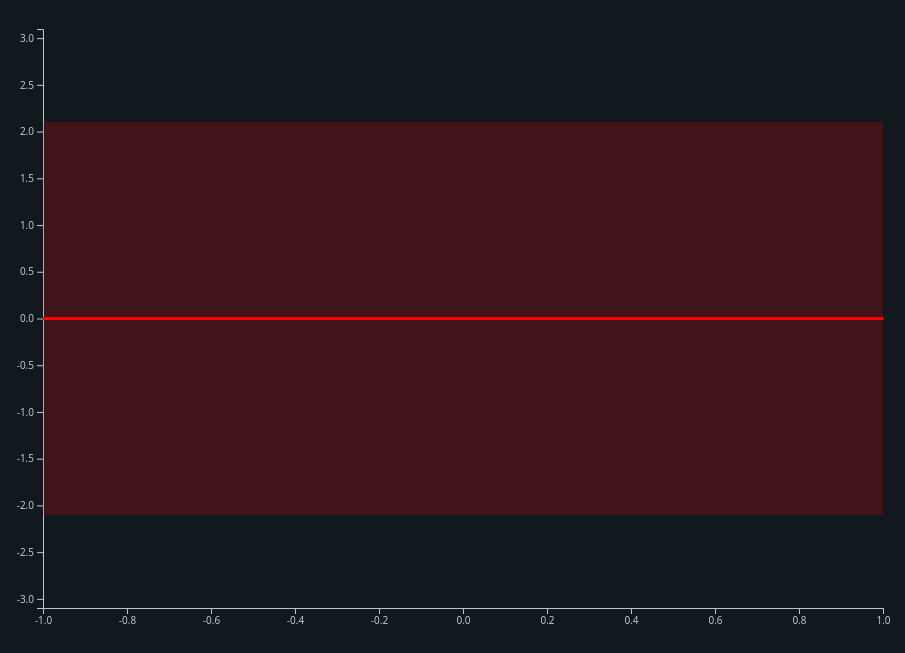
\includegraphics[width=0.2\textwidth]{../imgs/observing.png}
  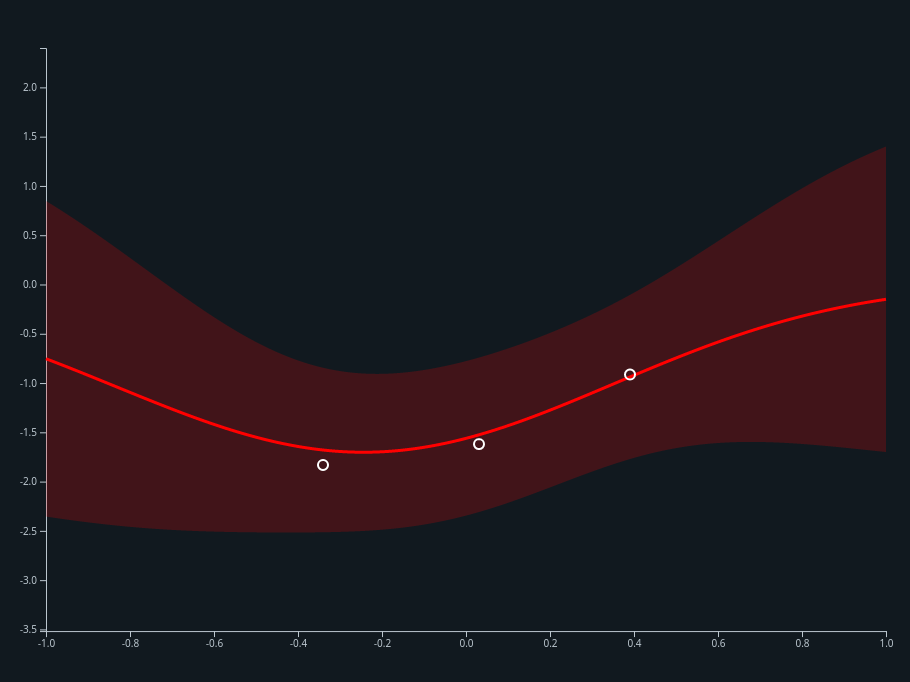
\includegraphics[width=0.19\textwidth]{../imgs/observed.png}
  \caption{Sampling from the GP.}
\end{figure}

Additionally, the tool provides a useful feature that allows users to gain insights into the marginal distribution of a specific $x$ point. By hovering over any vertical line on the chart, users can access information about the corresponding marginal distribution. This feature enhances the understanding of individual data points and their uncertainty estimates, enabling users to assess the impact of specific inputs on the overall model predictions.

\subsection{Choose between kernels}

The Gaussian Processes Visual Tool offers users the flexibility to choose from a variety of kernels for modeling the data. The tool supports several commonly used kernels, including the Radial Basis Function (RBF), Matern 5/2, Matern 3/2, Periodic, Linear, and Cosine kernels. Users can select their preferred kernel from this list, allowing them to tailor the model's characteristics to the specific dataset and desired assumptions.

Furthermore, the tool enables users to customize the kernel hyperparameters and the noise variance. Users can specify the values of the kernel hyperparameters to control aspects such as the smoothness, periodicity, or linearity of the underlying function. Additionally, they can adjust the noise variance to account for the level of uncertainty or noise present in the data.


\begin{figure}[H]
  \centering
  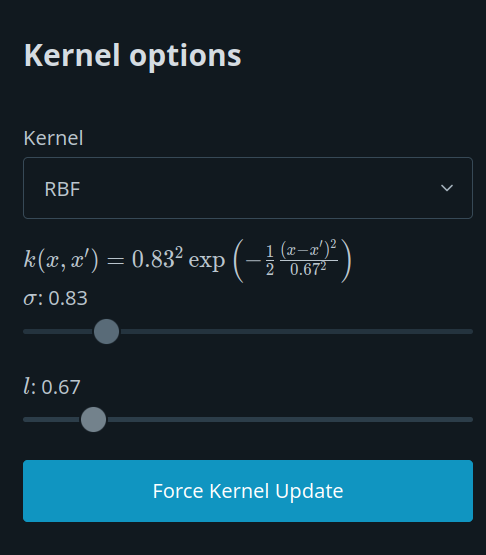
\includegraphics[width=0.20\textwidth]{../imgs/kernel-1.png}
  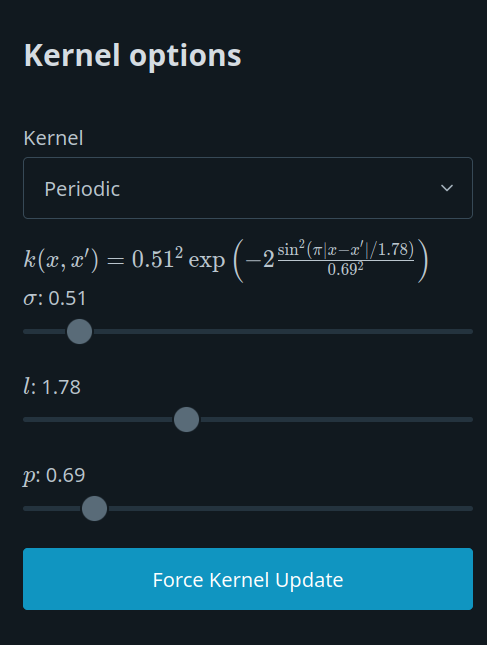
\includegraphics[width=0.18\textwidth]{../imgs/kernel-2.png}
  \caption{Changing kernels.}
\end{figure}

To assist users in optimizing the kernel hyperparameters, the tool provides a dedicated button that initiates the optimization process using the marginal likelihood. This feature automatically searches for the optimal values of the hyperparameters based on the given dataset, enhancing the modeling accuracy and facilitating the model selection process.

\subsection{Setting custom configurations to the GP}

The Gaussian Processes Visual Tool allows users to further customize the configurations of the GP model according to their specific requirements. The tool supports the following configurations:

  \begin{itemize}
    \item \textbf{Number of inducing points -} Users can specify the number of inducing points, which affects the granularity and complexity of the model. Adjusting this parameter allows users to control the trade-off between model accuracy and computational efficiency.
    \item \textbf{Starting and ending $x$ values -} Users have the flexibility to define the range of $x$ values to be considered in the GP model. This feature enables users to focus on specific regions of interest within the dataset and tailor the model's predictions accordingly.
    \item \textbf{Likelihood variance -} Users can set the likelihood variance, which represents the uncertainty or noise level in the observed data. Modifying this parameter helps capture the noise characteristics of the dataset and refine the model's predictions.
  \end{itemize}

\begin{figure}[H]
  \centering
  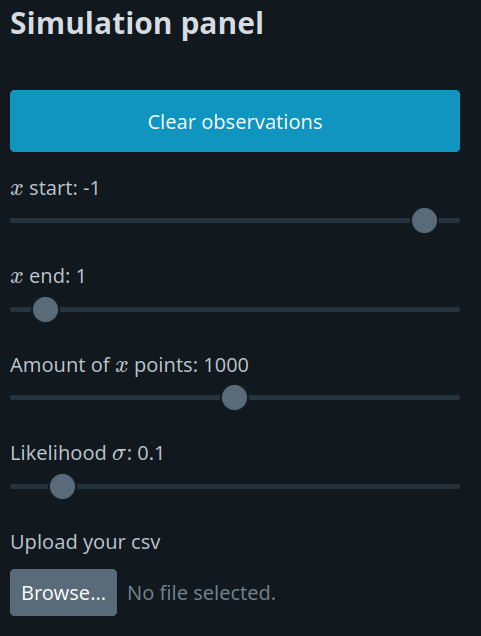
\includegraphics[width=0.30\textwidth]{../imgs/simulation.png}
  \caption{Simulation options}
\end{figure}


\begin{itemize}
  \item \textbf{Uploading your own data -} The tool offers the convenience of uploading custom datasets. Users can upload their data in a CSV file format with two columns: $x$ and $y$. This capability allows users to work with their own data and explore the behavior of the GP model on real-world datasets.
\end{itemize}

\section{Implementation Details}

In this section we are going to describe the implementation details of the Gaussian Processes Visual Tool. We will describe the main components of the tool and how they interact with each other.

\subsection{Frontend}

The frontend is built using Svelte and D3.js. Svelte is a JavaScript framework for building user interfaces. It provides a simple and intuitive way to create reactive components and manage state. D3.js is a JavaScript library for data visualization. It provides a wide range of tools for creating interactive charts and visualizations. The frontend is responsible for rendering the user interface and handling user interactions. It communicates with the backend to retrieve data and model updates.

\subsection{Backend}

The backend is built using Flask, a Python web framework. Flask provides a simple and flexible way to create web applications. The backend is responsible for handling data preprocessing, model training, and the flow of information between the frontend and backend components. It communicates with the frontend to receive user interactions and model updates. It also communicates with GPyTorch to train the GP model and make predictions. The data is sent from and to the frontend in JSON format by HTTP requests.

\subsection{GPyTorch}

GPyTorch is a Gaussian Process library for PyTorch. It provides a wide range of GP models and inference methods. It also provides a flexible and efficient way to define custom GP models. The Gaussian Processes Visual Tool uses GPyTorch to train the GP model and make predictions. It also uses GPyTorch to compute the marginal likelihood and optimize the kernel hyperparameters.

\subsection{Running the tool}

All code and documentation for the Gaussian Processes Visual Tool can be found on GitHub. The tool can be run locally by cloning the repository \url{https://github.com/adamesalles/gp-visual-tool}. There are some problems on deploying it online, but soon it will be available in a website.

\subsection{User Interface and User Experience}

Everything was meant to be simple and intuitive. The user interface is clean and easy to use. All values are set by sliders and the user can see the changes in real time. Some buttons are available to make the user experience even better. All styles are based on good practices and the user can easily understand what is happening. And, of course, you don't have to scroll to see everything.

\section{Conclusion}
In this paper, we introduced the Gaussian Processes Visual Tool, an interactive and flexible tool for visualizing Gaussian Processes (GPs). Leveraging the capabilities of Svelte, D3.js, Flask, and GPyTorch, the tool offers a user-friendly interface that can be adapted to various use cases. With its comprehensive set of functionalities, the tool empowers users to explore, understand, and teach GPs effectively.

The Gaussian Processes Visual Tool provides a seamless and interactive visualization experience for GPs. By leveraging the power of Svelte and D3.js, users can intuitively interact with the visualizations, make observations, and witness real-time updates of the posterior distribution and model predictions. This dynamic interaction enhances users' understanding of how observations impact the model and allows them to gain insights into the underlying patterns and uncertainties.

Furthermore, the tool serves as an educational resource, enabling users to teach and demonstrate the advantages of GPs over traditional regression methods. By providing a visual representation of GPs, users can showcase the non-parametric nature of GPs, their ability to capture complex relationships, and their probabilistic nature, which provides uncertainty estimates for predictions.

The Gaussian Processes Visual Tool is available on GitHub, providing an open-source platform that can be run locally. Its flexibility allows users to adapt it to their specific needs and datasets, facilitating research, experimentation, and practical applications of GPs. The availability of the tool on a popular open-source platform ensures its accessibility and fosters collaboration among researchers and practitioners.

In conclusion, the Gaussian Processes Visual Tool offers an intuitive and interactive solution for visualizing and understanding GPs. With its powerful visualization capabilities, educational potential, and adaptability, the tool contributes to the advancement and wider adoption of Gaussian Processes in various domains. We encourage researchers and practitioners to explore and leverage the tool to unlock the potential of GPs and gain deeper insights into complex data.


\subsection{Future work}

By addressing the following future work aspects, the Gaussian Processes Visual Tool can further expand its capabilities, flexibility, and usability, empowering users to explore and analyze GP models more comprehensively.

\begin{itemize}
  \item \textbf{Add more visualizations -} Currently, the Gaussian Processes Visual Tool provides visualizations of the posterior distribution and model predictions. In future work, additional visualizations can be incorporated, such as a heatmap of the covariance matrix. This visualization would provide insights into the correlations between different input variables, helping users understand the relationships within the data and their impact on the GP model.

  \item \textbf{Add more kernels -} The tool currently supports a range of kernel functions for GP modeling. To enhance its flexibility and modeling capabilities, future work can focus on expanding the selection of kernels. This would allow users to explore different modeling assumptions and capture a wider range of patterns and structures in the data.
  
  \item \textbf{Include export options -} To facilitate the use of the tool and enable further analysis, future work can incorporate export options. Users could have the ability to export visualizations, model parameters, and results in various formats, such as images, CSV files, or other common data formats. This would enable users to save and share their findings, integrate them into reports or presentations, or further analyze the results using external tools.

  \item \textbf{Make it run on GPU by default -} GP inference can be computationally demanding, especially for large datasets. To improve the tool's performance, future work can explore the option of running the computations on a GPU by default. Leveraging the parallel processing capabilities of GPUs would significantly accelerate the inference process, allowing users to work with larger datasets and complex models more efficiently.
  
  \item \textbf{Deploy it to a server -} Currently, the tool is available for local use. Future work can involve deploying the Gaussian Processes Visual Tool to a server, making it accessible via a web interface. This would enable users to access the tool remotely, collaborate with others, and utilize its functionalities without the need for local installation. Server deployment would also facilitate continuous updates and improvements to the tool.

  \item \textbf{Add math explanations to the tool -} To enhance user understanding, future work can focus on incorporating math explanations directly into the tool. This could involve providing tooltips or annotations that explain the mathematical concepts and formulas used in Gaussian Processes. By providing contextual explanations within the tool, users would gain a deeper understanding of the underlying principles and assumptions.

  \item \textbf{ Operations between kernels -} Gaussian Processes allow for combining and manipulating different kernel functions to create more complex models. Future work can explore the addition of operations between kernels within the tool. Users could have the ability to perform operations such as addition, multiplication, or composition of kernels, enabling them to create custom kernels that capture specific relationships and structures in the data.
\end{itemize}



%% if specified like this the section will be committed in review mode
\acknowledgments{
  The author extends heartfelt gratitude to Luiz Max Fagundes de Carvalho, his advisor, for being an exceptional mentor and friend throughout his undergraduate studies. Luiz Max introduced the author to the world of Gaussian Processes and statistics, providing invaluable guidance and inspiration. 

  Special thanks go to the author's friends Caio Lins, Tulio Koneçny, and Juan Belieni for their unwavering support and enriching discussions. Their contributions and encouragement have played a significant role in shaping the author's ideas and refining the Gaussian Processes Visual Tool.

  The author would also like to express appreciation to Prof. Jorge Poco for the continuous support and insightful guidance as the lecturer of the Visual Data Analysis course. The author is grateful for the opportunity to work on the Gaussian Processes Visual Tool as part of this course.
}

\bibliographystyle{unsrt}
% \bibliographystyle{abbrv-doi}
% \bibliographystyle{abbrv-doi-narrow}
%\bibliographystyle{abbrv-doi-hyperref}
%\bibliographystyle{abbrv-doi-hyperref-narrow}

\bibliography{template}
\end{document}

